
\chapter[Application for controlling a robot via SSVEP]{Application for controlling\\ a robot via SSVEP}
\label{sec:SSVEP_BCI}

The aim of this chapter is to describe the \gls{SSVEP}-based \gls{BCI} designed as a practical part of this thesis. The \gls{BCI} is written in Python 2.7 and the code is accessible from Github repository, see appendix~\ref{sec:code} for details. The \gls{BCI} requires only Emotiv EPOC headset and a computer with Windows operating system, no specific hardware like digital signal processors or \glspl{LED} are used.

\section{Controlling a robot with the application}

This section describes how the \gls{BCI} can be used to control a robot. Each \gls{target} in the \gls{BCI} can be used as one command for the robot. The robot can be controlled by looking at different \glspl{target} on the computer screen in certain sequence, depending on which command should be given to the robot. Then the \gls{BCI} tries to identify which \gls{target} is being looked at and translates the results into commands for the robot. The \glspl{target} could be designed for example as shown in figure~\ref{fig:arrow_stimuli}.

\begin{figure}[h]
	\centering
	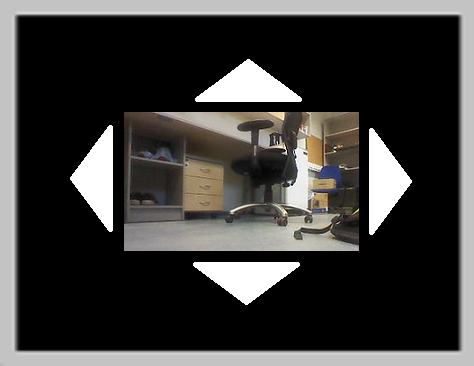
\includegraphics[width=0.8\textwidth]{arrows_stream.png}
	\caption{Stimuli locations on the screen for controlling a robot. The picture in the middle represents camera's video stream.}
	\label{fig:arrow_stimuli}
\end{figure}

The robot\footnote{https://github.com/kuz/Garage48-PiTank} used for testing the application has five possible commands: move forward, move backward, turn left, turn right and stop. The robot can execute one command at a time, meaning that it is not possible to move forward and turn left or right at the same time. If the robot is moving forward and receives a command to turn left, the moving forward will stop and the robot starts to turn left. See figure~\ref{fig:robot} for a picture of the robot used for testing the application.

\begin{figure}[h]
	\centering
	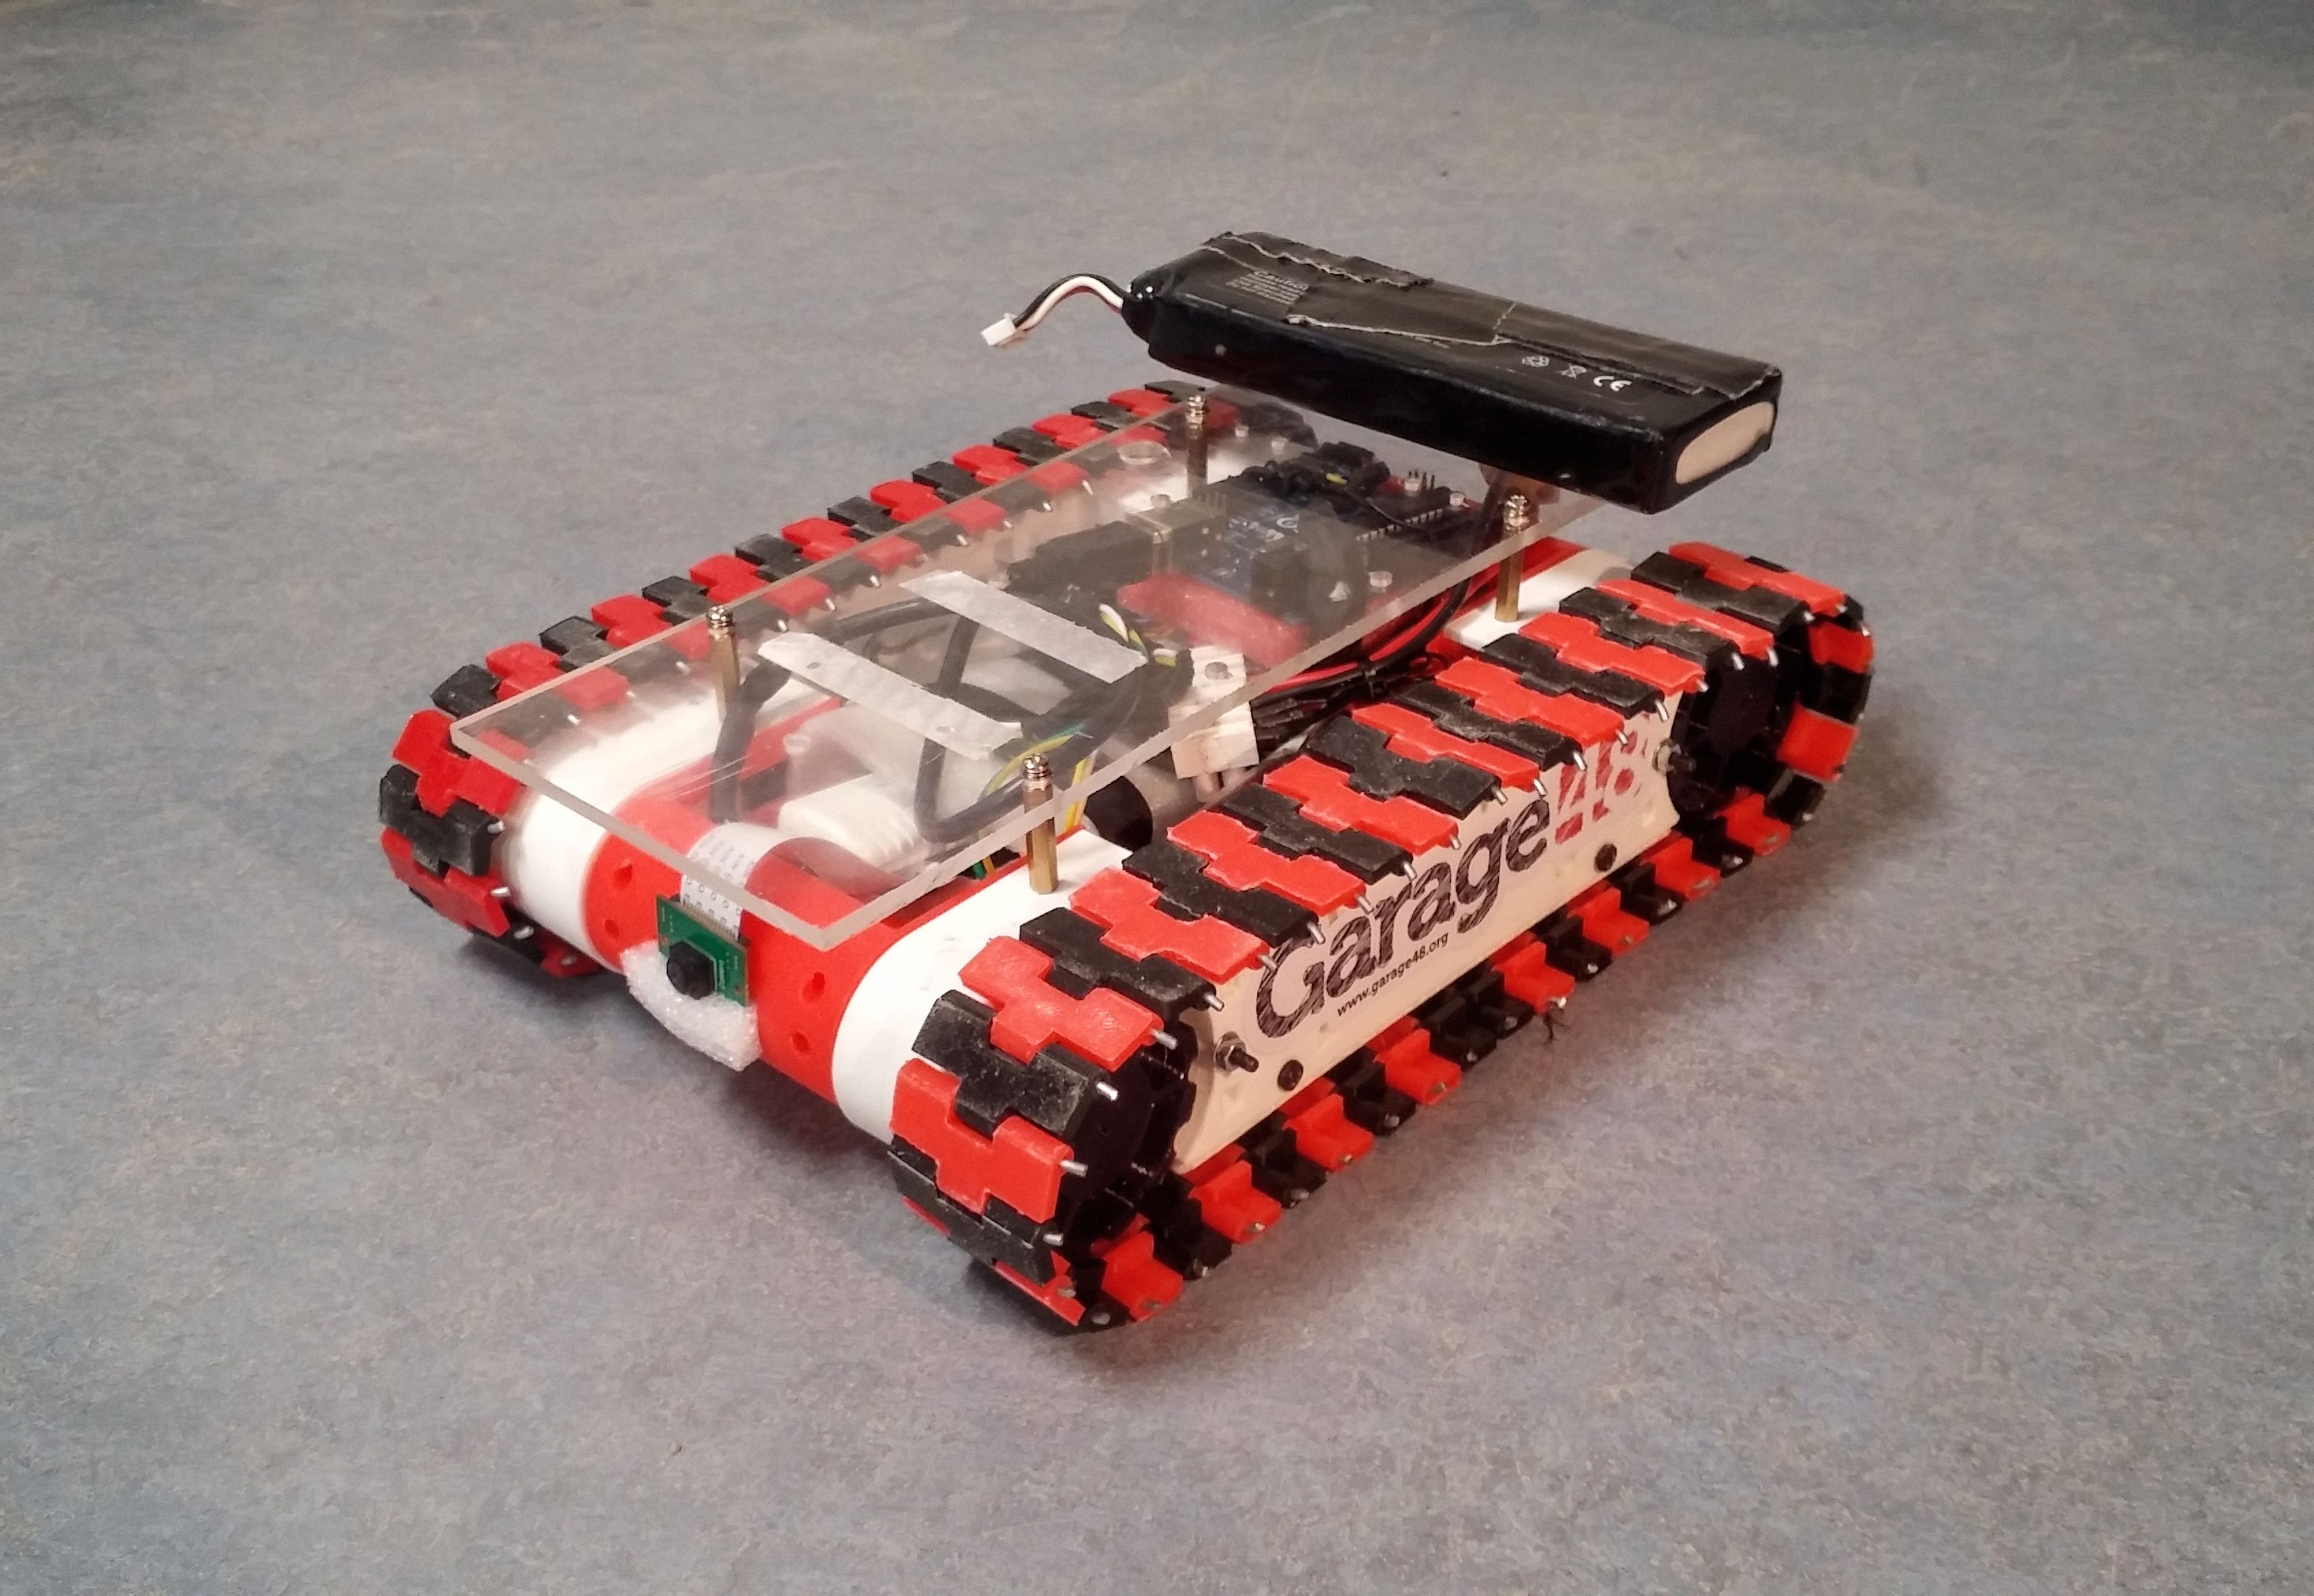
\includegraphics[width=0.6\textwidth]{robot.jpg}
	\caption{The robot used for testing the application.}
	\label{fig:robot}
\end{figure}

The robot has a camera on it and thus it is possible to see the camera's videos stream on the computer screen when controlling the robot with the application. The picture in the middle of the screen as shown in figure~\ref{fig:arrow_stimuli} represents the video stream.

The flowchart of the \gls{BCI} can be seen in figure~\ref{fig:whole_bci}. The brain and the Emotiv EPOC headset were discussed in the first chapter. The \glspl{target} and \gls{feature extraction} methods of the \gls{BCI} along with the signal processing techniques were discussed in the second chapter. The details of the actual implementation of the signal pipeline and the novel target identification method will be discussed in sections~\ref{sec:signal_pipeline} and \ref{sec:identification} respectively.

\begin{figure}[h!]
	\centering
	\tikzstyle{decision} = [diamond, draw, fill=blue!20,
    text width=6em, text badly centered, inner sep=0pt]
\tikzstyle{block} = [rectangle, draw, fill=blue!20,
    text width=6em, text centered, rounded corners, minimum height=4em]
\tikzstyle{line} = [draw, very thick, color=black!50, -latex']
\tikzstyle{cloud} = [draw, ellipse,fill=red!20, 
    minimum height=2em]
\tikzstyle{noArrow} = [draw, very thick, color=black!50]

\begin{tikzpicture}[scale=2, node distance = 4cm, auto]
	% Nodes
	\node (monitor) {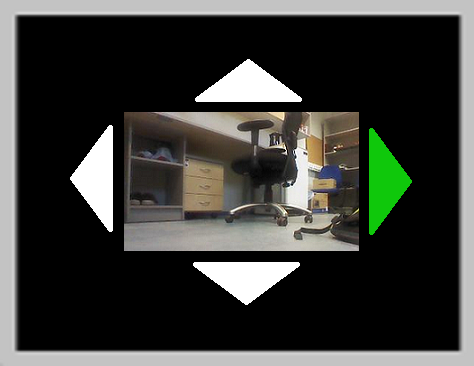
\includegraphics[width=4cm]{arrows_chosen.png}};
	\node [below of=monitor] (brain) {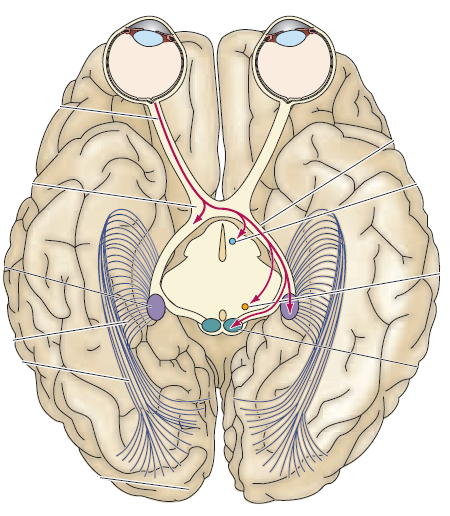
\includegraphics[width=2.5cm]{visual_pathway2.png}};
	%\node [below of=brain, node distance=2cm] {\includegraphics[width=1cm]{electrode.png}};
	\node [block, right of=brain] (emotiv) {Emotiv EPOC headset};
	\node [block, right of=emotiv] (processing) {signal processing};
	\node [block, right of=processing] (extraction) {feature extraction};
	\node [block, above of=extraction] (identification) {target identification};
	\node [left of=identification, node distance=6cm] (robot) {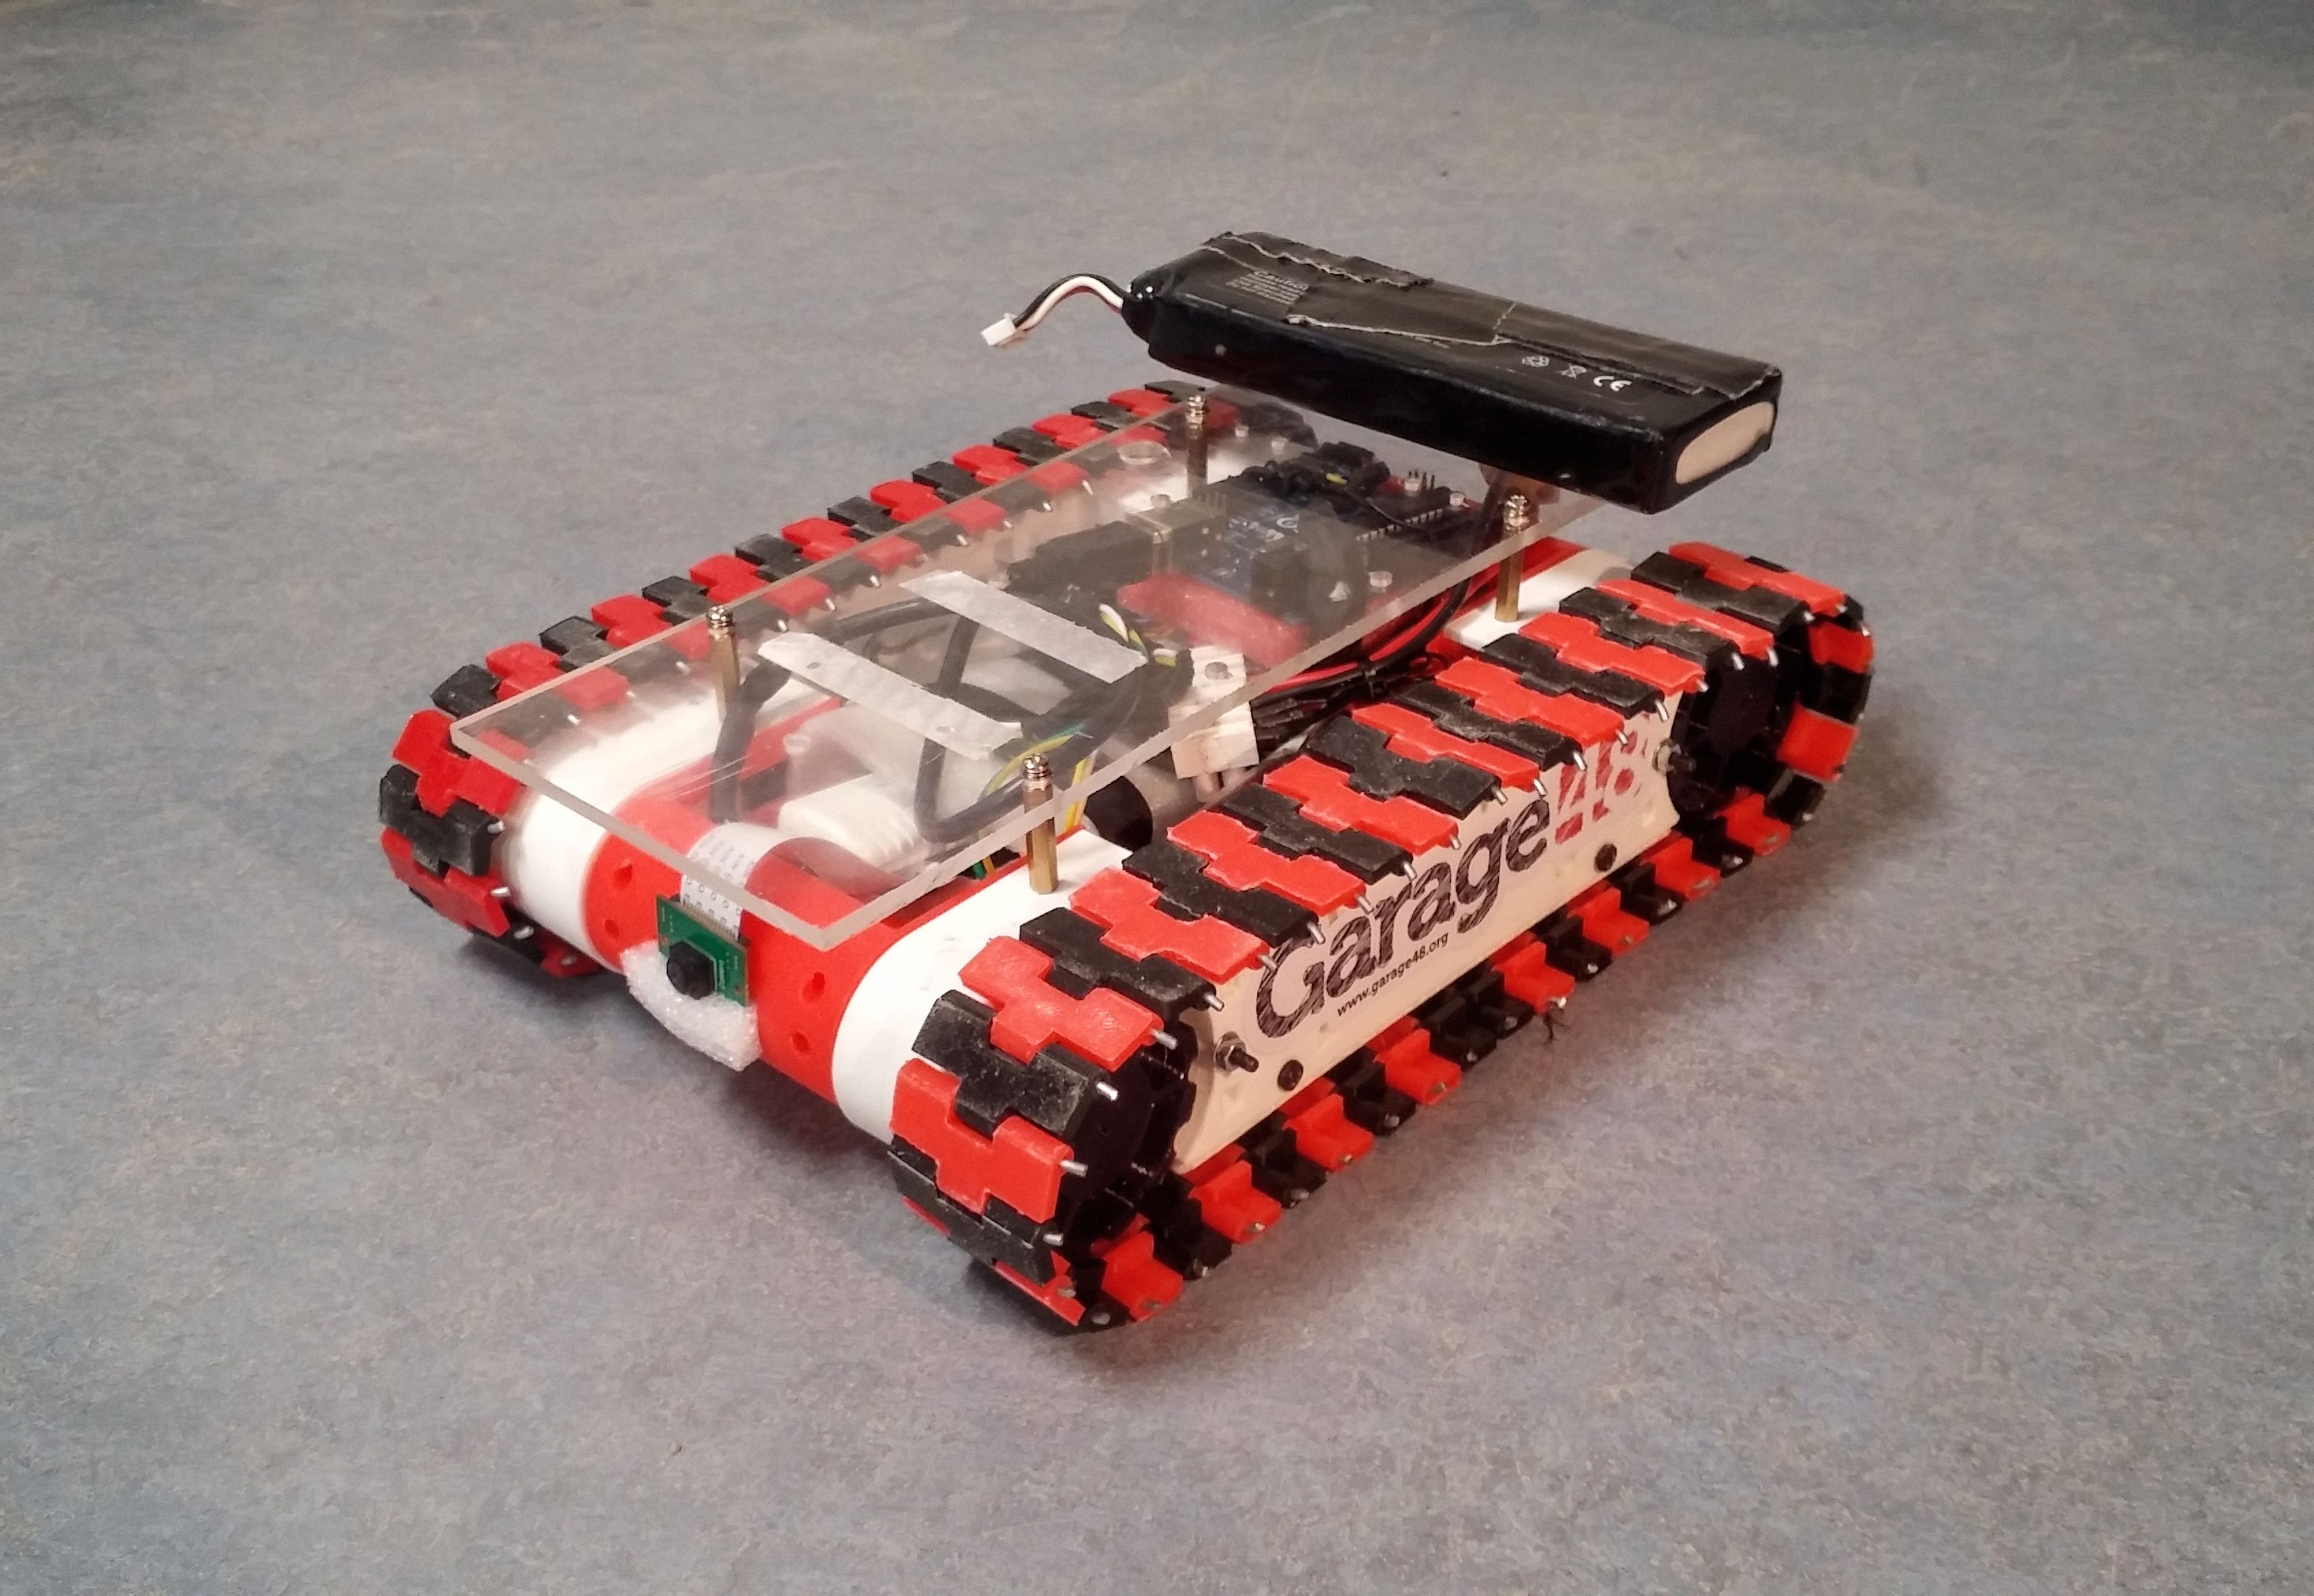
\includegraphics[width=4cm]{robot.jpg}};
	
	\coordinate [above of=robot, node distance=2cm] (dummy);
	\coordinate [left of=dummy] (dummyLeft);
	\coordinate [right of=dummy] (dummyRight);
	
	% Arrows
	\path [noArrow] (identification) -- (dummyRight);
	\path [noArrow] (dummyRight) -- node [color=black, pos=0.5, above] {visual and auditory feedback} (dummyLeft);
	\path [line] (dummyLeft) -- (monitor);
	\path [line] (identification) -- node [color=black, above] {command} (robot);
	\path [line] (extraction) -- (identification);
	\path [line] (processing) -- (extraction);
	\path [line] (emotiv) -- (processing);
	\path [line] (brain) -- (emotiv);
	%\path [line] (threshold) -- node [near start, color=black] {yes} (add);
	%\path [line] (dummyStopRight) -- (new);

\end{tikzpicture}

	\caption{Flowchart of the BCI.}
	\label{fig:whole_bci}
\end{figure}

The robot used in testing the application has very common commands---forward, back, left, right and stop. Therefore, if the \gls{BCI} proves to have sufficiently high \gls{target} detection speed and accuracy, then it could be adapted to other devices that can be controlled with similar commands.

\section{Overview of the application}
\label{sec:application}

As already mentioned, the application implements a communication channel between the brain and a robot, thus making it possible to send control commands to the robot. Brain activity is recorded using Emotiv EPOC and the recording is analysed with \gls{PSDA} and \gls{CCA} \gls{feature extraction} methods. The application is open-source, written in Python 2.7 and requires Windows operating system.

The application is divided into the following components:
\begin{itemize}
	\item\texttt{MainWindow} is the window through which a user can easily change the parameters of the signal pipeline, \gls{feature extraction} methods and \glspl{target} and control the flow of the application through \gls{GUI};
	\item\texttt{TargetsWindow} is the window on which the \glspl{target} are displayed;
	\item\texttt{Emotiv} is the class which receives the raw data from the Emotiv EPOC headset, decrypts the data and sends it to other components of the application;
	\item\texttt{Robot} is the code that sends commands to the robot after the signal has been analysed and result has been obtained;
	\item\texttt{Plot} is the code that can be used to plot the \gls{EEG} signal in real-time;
	\item\texttt{Extraction} is the code that analyses the signal using \gls{PSDA} and \gls{CCA} \gls{feature extraction} methods.
	\item\texttt{PostOffice} is the class that handles the communication between the components of the application.
\end{itemize}
There is instance one of each component except the \texttt{Plot} and the \texttt{Extraction}. The number of \texttt{Plots} and \texttt{Extractions} depends on how many plots the user wants to see or how many \gls{feature extraction} methods to use. Each plot and \gls{feature extraction} method can have different parameters. Having different parameters on different plots allows the user to compare how different signal processing affects the signal. Having different parameters on \gls{feature extraction} methods allows the user to compare how the parameters affect the performance of the \gls{BCI}. Furthermore, \gls{feature extraction} methods with different parameters can be used together to complement each other and work as a single \gls{feature extraction} method. Combining different \gls{feature extraction} methods to a single method is further discussed in section~\ref{sec:identification}. For graphical illustration of the components of the application see figure~\ref{fig:class_diagram}.

\begin{figure}[h!]
	\centering
	\tikzstyle{decision} = [diamond, draw, fill=blue!20,
    text width=4.5em, text badly centered, node distance=2.5cm, inner sep=0pt]
\tikzstyle{block} = [rectangle, draw, fill=blue!20,
    text width=5em, text centered, rounded corners, minimum height=4em]
\tikzstyle{line} = [draw, very thick, color=black!50]
\tikzstyle{cloud} = [draw, ellipse,fill=red!20,
    minimum height=2em]

\newcommand*{\ArrowLength}{2.0em}
\newcommand*{\MyRightArrow}[1][]{
    \tikz [-stealth, red, yshift=0.5ex, baseline] 
        \draw [-stealth, #1] (0,0) -- (\ArrowLength,0) ;
}

\begin{tikzpicture}[scale=2, node distance = 4cm, auto]
	% Nodes
	\node [block] (PostOffice) {\texttt{PostOffice}};
	\node [block, left of=PostOffice] (MainWindow) {\texttt{Main Window}};
	\node [block, right of=PostOffice] (TargetsWindow) {\texttt{Targets Window}};
	\node [block, below of=TargetsWindow, node distance=2cm] (Robot) {\texttt{Robot}};
	\node [block, below of=MainWindow, node distance=2cm] (MyEmotiv) {\texttt{Emotiv}};
	\node [block, above of=TargetsWindow, node distance=2cm] (Plot) {\texttt{Plot}};
	\node [block, above of=MainWindow, node distance=2cm] (Extraction) {\texttt{Extraction}};
	
	% Arrows
	\path [line] (PostOffice) -- node [pos=0.1, above, color=black] {1} node[pos=0.9, above, color=black] {1} (MyEmotiv);
	\path [line] (PostOffice) -- node [pos=0.1, above, color=black] {1} node[pos=0.9, above, color=black] {1} (TargetsWindow);
	\path [line] (PostOffice) -- node [pos=0.1, above, color=black] {1} node[pos=0.9, above, color=black] {1} (MainWindow);
	\path [line] (PostOffice) -- node [pos=0.1, above, color=black] {1} node[pos=0.9, above, color=black] {1} (Robot);
	\path [line] (PostOffice) -- node [pos=0.1, above, color=black] {1} node[pos=0.9, above, color=black] {n} (Plot);
	\path [line] (PostOffice) -- node [pos=0.1, above, color=black] {1} node[pos=0.85, above, color=black] {m} (Extraction);

\end{tikzpicture}

	\caption{Components of the application. Lines between the components represent connections through which the components communicate. The numbers show how many instances of the same component there can be.}
	\label{fig:class_diagram}
\end{figure}

The \texttt{PostOffice} class is important because each component is running on separate subprocess, meaning that each component has its own memory space. Thus it is not possible for the components of the application to communicate by for example writing to and reading from the same variable---their memory is separated---and therefore more complex type of communication has to be used. Alternative to using multiple processes or multiprocessing is using multiple threads or multithreading. Unlike processes, threads run in the same memory space but due to the limitations of the standard implementation of Python, threads cannot use multiple \glspl{CPU} or multiple \gls{CPU} cores at the same time while processes can.

Making use of multiple \gls{CPU} cores is important because calculating the \gls{power spectral density} and analysing the recorded signal using \gls{CCA} is computationally expensive and thus it might be necessary to divide the calculations between different \gls{CPU} cores to achieve optimal performance and use the \gls{BCI} in real-time. The Emotiv EPOC headset is constantly sending new data to the application and the application has to be able to finish analysing current data before receiving enough data for the next \gls{feature extraction}.

For the ease of use, the application has \gls{GUI}. See figure~\ref{fig:options_frame} for an example of the application's user interface. Multiprocessing is also important to avoid freezing of the whole application while one window of the \gls{GUI} is moved or resized. In case of moving a window, the window manager of Windows operating system freezes the subprocess which is updating the window. If the application is divided into subprocesses then only the subprocess which updates the window freezes, the rest of the application continues working.

The usage of multiple subprocesses is achieved by using multiprocessing module from Python 2.7 standard library. This module also provides connections that can be used for communication between the components of the application. In addition to the Python 2.7 standard library, the following libraries were used:
\begin{itemize}
	\item Emokit\footnote{https://github.com/openyou/emokit/tree/master/python/emokit} to access raw data from Emotiv EPOC headset;
	\item PsychoPy~\cite{psychopy} for designing visual stimuli and precise timing of the stimuli presentations;
	\item scikit-learn~\cite{scikit-learn} for calculating \gls{CCA} algorithm;
	\item SciPy and NumPy~\cite{scipy} for calculating other advanced mathematical algorithms, for example \gls{FFT};
	\item PyQtGraph\footnote{http://www.pyqtgraph.org} for real-time plotting of the data.
\end{itemize}

The most important part of the implementation of this application is that multiple \gls{feature extraction} methods complement each other when analysing \gls{EEG} recording.

\section{Signal pipeline of the application}
\label{sec:signal_pipeline}

As already discussed in the previous section, the application does not have one specific signal pipeline, but the parameters of the signal pipeline can be changed from the \gls{GUI}. This allows different configurations to be easily tested to find the best settings for controlling a robot and the best settings for different users. See figure~\ref{fig:signal_pipeline} for the flowchart of the application's signal pipeline.

\begin{figure}[h!]
	\centering
	\tikzstyle{decision} = [diamond, draw, fill=blue!20,
    text width=4.5em, text badly centered, node distance=2.5cm, inner sep=0pt]
\tikzstyle{block} = [rectangle, draw, fill=blue!20,
    text width=5em, text centered, rounded corners, minimum height=4em]
\tikzstyle{line} = [draw, very thick, color=black!50, -latex']
\tikzstyle{cloud} = [draw, ellipse,fill=red!20, node distance=3cm,
    minimum height=2em]

\begin{tikzpicture}[scale=2, node distance = 4cm, auto]
	% Nodes
	\node [cloud] (start) {start};
	\node [decision, below of=start] (wait) {wait for step packets};
	\node [block, right of=wait] (filter) {filter new signal segment};
	\node [cloud, right of=start] (stop) {stop};
	\node [block, right of=filter] (add) {add segment to signal};
	\node [decision, right of=add, node distance=4 cm] (length) {len(signal) \textgreater window length?};
	\node [block, below of=length] (delete) {delete first step packets};
	\node [block, left of=delete] (detrend) {make copy of signal and detrend it};
	\node [block, left of=detrend] (window) {window signal};
	\node [block, left of=window] (detect) {send signal to feature extraction};
	
	% Arrows
	\path [line] (start) -- (wait);
	\path [line] (wait) -- node [align=center, color=black, sloped, pos=1] {received\\"Stop"} (stop);
	\path [line] (wait) -- node [align=center, color=black, sloped] {received\\data} (filter);
	\path [line] (filter) -- (add);
	\path [line] (add) -- (length);
	\path [line] (length) -- node [near start, color=black] {yes} (delete);
	\path [line] (length) -- node [near start, color=black] {no} (detrend);
	\path [line] (detrend) -- (window);
	\path [line] (delete) -- (detrend);
	\path [line] (window) -- (detect);
	\path [line] (detect) -- (wait);
\end{tikzpicture}

	\caption{Flowchart of the application's signal pipeline.}
	\label{fig:signal_pipeline}
\end{figure}

As seen in figure~\ref{fig:signal_pipeline}, \texttt{length} is the \gls{window} length and it shows how long filtered signal is held in memory. \texttt{Step} on the other hand shows how many packets have to be received before trying to identify user's choice. If \texttt{step} is smaller than \texttt{length} then the \gls{window} is overlapping which means that some of the data that was used in previous \gls{feature extraction} will also be used in the next \gls{feature extraction}. If \texttt{step} is equal to \texttt{length}, then every consecutive \gls{feature extraction} uses only new data that has not been analysed by previous \glspl{feature extraction}. It would not make sense to use larger \texttt{step} than \texttt{length}, because then some of the data will not be analysed and in this case the \gls{target} detection would be slower.

After receiving \texttt{step} packets, the whole filtered signal will be first \glsdisp{detrend}{detrended} and then \glsdisp{window}{windowed}. \glsdisp{detrend}{Detrending} and \glsdisp{window}{windowing} were thoroughly discussed in sections~\ref{sec:detrend} and \ref{sec:window} respectively. Since some data is deleted and new data is added to the signal after every step, the \glsdisp{window}{windowing} cannot be performed only on the previously received signal segment, but has to be performed on the whole signal every time. \glsdisp{detrend}{Detrending} could be performed only on the previously received signal segment, but using it on the whole signal gives more possibilities since the same result as would be obtained by \glsdisp{detrend}{detrending} every new signal segment can be achieved by dividing the \glsdisp{detrend}{detrending} of the whole signal into segments with suitable length. In the application this division can be achieved by giving the \texttt{break} parameter which shows how many breakpoints to use that divide the signal into equal length segments for \glsdisp{detrend}{detrending}.

There are more signal pipeline settings that can be changed through the \gls{GUI} of the application and now a brief overview of these settings will be given. See figure~\ref{fig:options_frame} for illustration of the application's \gls{GUI} for choosing signal pipeline components and parameters.

\begin{figure}[h]
	\centering
	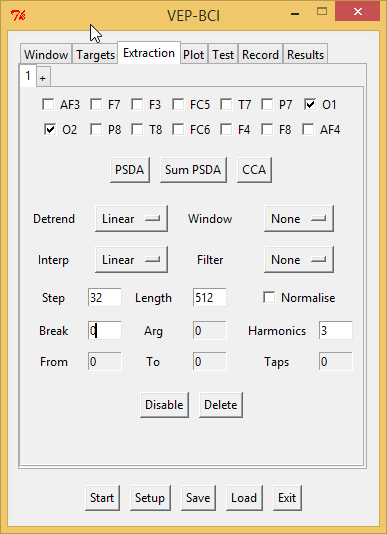
\includegraphics[width=0.6\textwidth]{options_frame.png}
	\caption{The user interface for choosing signal pipeline options.}
	\label{fig:options_frame}
\end{figure}

The explanation of the signal pipeline settings is the following:
\begin{enumerate}
	\item \texttt{\Gls{detrend}} is either linear, constant or none. None means that \glsdisp{detrend}{detrending} is not used. Linear means that linear trend is removed from the raw signal; constant means that constant trend is removed from the raw signal. \glsdisp{detrend}{Detrending} was more thoroughly discussed in section~\ref{sec:detrend}.
	\item \texttt{\Gls{window}} is either hann, hamming, blackman, keiser, bartlett or none. None means that \gls{window} function is not used. Other options are standard signal processing \gls{window} functions. \glsdisp{window}{Windowing} was more thoroughly discussed in section~\ref{sec:window}.
	\item \texttt{\glsdisp{interpolation}{Interp}} is either linear, nearest, zero, slinear, quadratic or cubic. See SciPy documentation\footnote{https://docs.scipy.org/doc/scipy/reference/generated/scipy.interpolate.interp1d.html} for more information. \Gls{interpolation} was more thoroughly discussed in section~\ref{sec:interpolate}.
	\item \texttt{Filter} is either high-pass, low-pass, band-pass or none. None means that filtering is not used. High-pass filter means that frequencies lower than the given value are removed from the signal. Similarly, low-pass filter removes frequencies higher than the given value. Band-pass filter takes two values and removes frequencies that are not in the given range. See SciPy documentation\footnote{http://docs.scipy.org/doc/scipy/reference/generated/scipy.signal.firwin.html} for more information. 
	\item \texttt{Step} shows how many packets have to be received before trying to identify user's choice. For example, if \gls{sampling rate} is \SI{128}{Hz} and step is 64 then the \gls{feature extraction} algorithms are executed after every $\frac{64}{\SI{128}{Hz}}=0.5$ seconds.
	\item \texttt{Length} is the length of the window. Length shows the number of packets on which the \gls{feature extraction} algorithms are executed. For example, if \gls{sampling rate} is \SI{128}{Hz} and length is 512 then the \gls{feature extraction} algorithms are performed on the last $\frac{512}{\SI{128}{Hz}}=4$ seconds of data.
	\item \texttt{Break} is the number of breakpoints used when \glsdisp{detrend}{detrending} the signal. The breakpoints will be equally spaced. If the number of breakpoints is 1, then the breakpoint will be in the middle of the signal and the trend will be removed separately from the first half of the signal and the second half of the signal.
	\item \texttt{Arg} is the beta argument for kaiser window. See NumPy documentation for details\footnote{http://docs.scipy.org/doc/numpy/reference/generated/numpy.kaiser.html}.
	\item \texttt{Normalise} shows whether to normalise the estimated \gls{power spectral density} as in equation~\ref{eq:norm_SNR} or not.
	\item \texttt{From} and \texttt{to} are the frequencies used to specify which frequencies are removed and which not. From shows the lowest frequency that is passed, lower frequencies than the value will be removed; to shows the highest frequency that is passed, higher frequencies than the value will be removed.
	\item \texttt{Taps} shows the number of taps or the length of the filter. See SciPy documentation\begin{NoHyper}\addtocounter{footnote}{-2}\footnotemark\addtocounter{footnote}{1}\end{NoHyper} for details.
\end{enumerate}

Since the application has \gls{GUI} and many parameters that can be easily tested, this application can be a good tool to compare how different signal pipelines affect the detection of \glspl{SSVEP}.

\section{Target identification method}
\label{sec:identification}

This section describes the \gls{target} identification method used in this application. As is the case with the signal pipeline, this application actually does not have one specific \gls{feature extraction} method, but the \gls{feature extraction} method can be changed and a combinations of different \gls{feature extraction} methods can be used. To the best of the author's knowledge, combining different \gls{feature extraction} methods while using only \gls{SSVEP} neuromechanism has not been used before.

Currently the application has three different \gls{feature extraction} methods that can be combined: widely known \gls{PSDA} and \gls{CCA} method and a method that is similar to the \gls{PSDA} method but the estimated \gls{power spectral density} is calculated not for each signal obtained from different channels but for the sum of all the signals from different channels. If only one channel is used, then this method works exactly the same as standard \gls{PSDA} method. In the \gls{GUI}, this method is called \texttt{sum \gls{PSDA}} method. Using this method makes sense, because \gls{FFT} is linear, meaning that the result will be the same if first the signals are summed up and then the \gls{power spectral density} is estimated and if first the \gls{power spectral density} is estimated separately for each channel and then the \gls{power spectral density} estimates for each channel are summed up.

Unlike the sum \gls{PSDA} method, the standard \gls{PSDA} method calculates separate results for each channel. Both methods send the results to the \texttt{PostOffice} separately for each \gls{harmonic}. Which \glspl{harmonic} are used for the detection of which \gls{target} can be changed in the \gls{GUI}. It is also possible to get the result for the sum of different \glspl{harmonic}. The \gls{CCA} method is different from the \gls{PSDA} methods as it gives always only one result, even if multiple channels and multiple harmonics are used.

Since multiple \gls{feature extraction} methods can be used together and some \gls{feature extraction} methods give more than one result, each \gls{feature extraction} result is given a certain weight which shows how much this result affects the final decision. For example, if \gls{CCA} and sum \gls{PSDA} method are used together and from the sum \gls{PSDA} results the result of the first \gls{harmonic} and the result of the sum of all used \glspl{harmonic} are used for each \gls{target}, then the weights could be 1 for each sum \gls{PSDA} result and 2 for \gls{CCA} result. Then the \gls{target} could be finally chosen for example if the sum of the weights for a \gls{target} is at least 3. This means actually that \gls{target} is chosen only if \gls{CCA} method chooses a \gls{target} and at least one of the sum \gls{PSDA} results is the same. This case could be easily implemented without using weights, but when using more \gls{feature extraction} methods, the conditions for choosing a target without using the weights will get more complicated and thus it is easier to use the weights to make the final decision.

To further improve the performance of the \gls{BCI}, not only the weights of the last results, but the weights of multiple previous results are used to make the decision. Thus the condition would not be that if the sum of the weights of the last results is at least 3, but for example the sum of the weights of the three previous results is at least 9. If there are multiple \glspl{target} that satisfy the condition, then the \gls{target} with higher sum of the weights of the previous results is chosen. This case is not possible in the previously given example, since all the results always correspond to one \gls{target}. In the previous example the maximum sum of weights for one set of results is 4, therefore the sum of weights for the last three sets of results is $4\cdot 3=12$. If the condition is that this sum has to be higher than 9, then the maximum sum of weights for another \gls{target} is $12-9=3$.

Finally, the \gls{target} is chosen if $n$ out of $m$ previous results that were obtained by comparing the sum the weights of $k$ previous results are the same. See figure~\ref{fig:target_identification} for graphical illustration of the \gls{target} identification method.

\begin{figure}[h!]
	\centering
	\tikzstyle{decision} = [diamond, draw, fill=blue!20,
    text width=6em, text badly centered, inner sep=0pt]
\tikzstyle{block} = [rectangle, draw, fill=blue!20,
    text width=6em, text centered, rounded corners, minimum height=4em]
\tikzstyle{line} = [draw, very thick, color=black!50, -latex']
\tikzstyle{cloud} = [draw, ellipse,fill=red!20, 
    minimum height=2em]
\tikzstyle{noArrow} = [draw, very thick, color=black!50]

\begin{tikzpicture}[scale=2, node distance = 4cm, auto]
	% Nodes
	\node [cloud] (start) {start};
	
	\coordinate [below of=start, node distance=5cm] (dummyStart);
	\coordinate [left of=dummyStart, node distance=2cm] (dummyStartLeft);
	
	\node [block, left of=start] (wait) {wait for $k$ results};
	\node [block, below of=wait, node distance=3cm] (calculate) {calculate the sum of the weights of $k$ last results};
	\node [decision, right of=calculate] (threshold) {is sum \textgreater= threshold?};
	\node [block, right of=threshold] (add) {add corresponding target to list};
	\node [decision, below of=add] (del) {more than $n$ targets in the list?};
	\node [block, left of=del] (remove) {delete the first target from the list};
	
	\coordinate [below of=remove, node distance=2cm] (dummyDel);
	\coordinate [right of=dummyDel, node distance=2cm] (dummyDelRight);
	\coordinate [left of=dummyDel, node distance=2cm] (dummyDelLeft);
	
	\node [decision, left of=remove] (final) {at least $m$ same targets in the list?};
	\node [block, left of=final] (correct) {choose the target with the most occurrences};
	\node [decision, above of=correct] (new) {wait for next results};
	\node [cloud, above of=new, node distance=3cm] (stop) {stop};
	
	\coordinate [below of=stop, node distance=5cm] (dummyStop);
	\coordinate [right of=dummyStop, node distance=2cm] (dummyStopRight);
	
	%\node [block, right of=start] (receive) {receive result(s) from feature extraction};
	%\node [decision, below of=length, node distance=2.7cm] (received) {received "Stop"?};

	
	% Arrows
	\path [noArrow] (threshold) -- node [near start, color=black] {no} (dummyStartLeft);
	\path [noArrow] (dummyStartLeft) -- (dummyStopRight);
	\path [line] (threshold) -- node [near start, color=black] {yes} (add);
	\path [line] (dummyStopRight) -- (new);
	\path [line] (start) -- (wait);
	\path [line] (wait) -- (calculate);
	\path [line] (calculate) -- (threshold);
	\path [line] (add) -- (del);
	\path [line] (del) -- node [near start, color=black, above] {yes} (remove);
	\path [line] (remove) -- (final);
	\path [line] (final) -- node [near start, color=black, above] {yes} (correct);
	\path [line] (final) -- node [near start, color=black] {no} (new);
	\path [line] (correct) -- (new);
	\path [line] (new) -- node [near start, color=black, align=right] {received\\ results} (calculate);
	\path [line] (new) -- node [near start, color=black, align=center] {received\\ "Stop"} (stop);
	\path [noArrow] (del) -- node [near start, color=black] {no} (dummyDelRight);
	\path [noArrow] (dummyDelRight) -- (dummyDelLeft);
	\path [line] (dummyDelLeft) -- (final);
	
	%\path [line] (received) -- node [near start, color=black] {yes} (stop);
	
\end{tikzpicture}

	\caption{Flowchart of the application's target identification.}
	\label{fig:target_identification}
\end{figure}

%One way to identify user's choice with standard \gls{PSDA} method is to choose a command only if results of all the different channels are the same. If all the methods do not give the same result, it is assumed that the signal was too noisy and the decision could not be made. In this case the application waits for new data.

%All \gls{feature extraction} methods used in the application can be combined. In case of combining methods, the \gls{target} choosing algorithm is similar to the standard \gls{PSDA} method---all the methods have to give the same result. Currently the \gls{target} choosing method cannot be changed from the user interface. If different \gls{target} choosing method is needed, then the code has to be changed.

It is easy to modify \gls{target} identification method by changing the code in \texttt{handleFreq-\break Message} method in \texttt{PostOffice.py}. This method receives the results of the \gls{feature extraction} methods through a connection similarly to the data accessing code discussed in section~\ref{sec:different_devices}. The results have already been organised into different data structures. %There are results per each method, results per each signal pipeline, all the results counted and other data structures to make it easier to further develop the application.

It is also worth mentioning that different \gls{feature extraction} methods can have different signal pipelines. For example it would not make sense to \gls{window} a signal that is later analysed using \gls{CCA}, but \glsdisp{window}{windowing} could be beneficial if the \gls{power spectral density} of the signal is later estimated analysed using \gls{PSDA} method. Thus the application has the functionality to use multiple signal pipelines with different options, which gives even more flexibility.

Using \gls{PSDA} and \gls{CCA} method together makes the \gls{target} identification more accurate, because finally the \gls{target} is chosen only if different methods give the same result. If one of the methods makes a mistake and gives a wrong result, then the other method might still give the correct result. It is less probable for two methods to make the same mistake at the same time than for one method to make a mistake. Using these two methods together makes sense, because these methods analyse the \gls{EEG} signal from two different aspects---one uses time-domain representation, the other uses frequency-domain representation.

To further improve this method, the phase information from the \gls{frequency spectrum} that is currently being discarded could also be used. One possible usage would be to design \gls{CCA} method \glspl{reference signal} with correct phase. Currently both sine and cosine waves are used to achieve optimal minimum correlation as discussed in section~\ref{sec:CCA}. But even without this improvement, combining these methods already improves the performance of the \gls{BCI}.

\section{Using the application with other EEG devices}
\label{sec:different_devices}

Although the application was written for Emotiv EPOC, it can be used with other \gls{EEG} devices too if it is possible to access the data of these devices with Python script. As discussed in section~\ref{sec:application}, the communication between the data accessing code and the rest of the application is implemented using Python multiprocessing module. The data accessing code runs on separate process and communicates with the rest of the application by sending messages through multiprocessing connection. It sends raw data through the connection and receives messages like "Setup", "Start", "Stop" and "Exit". Each of the received messages should lead to calling a specific function. If the received message is
\begin{itemize}
	\item "Setup", then the object should get internally ready to start sending data;
	\item "Start", then the object should start sending the data;
	\item "Stop", then the object should stop sending the data;
	\item "Exit", then all the needed clean up procedures should be executed, because the application is closing.
\end{itemize}

The easiest way to start using different headset with the application is changing the code in \texttt{MyEmotiv.py}. The constructor of \texttt{MyEmotiv} class has to take one argument. This argument is the object that handles the communication between different processes. The last line in the constructor of \texttt{MyEmotiv} should call the argument's \texttt{waitMessages} method, which waits until it receives one of the previously discussed messages. The \texttt{waitMessages} method takes arguments which are the functions that are called when corresponding message is received. By replacing these methods in \texttt{MyEmotiv} class, it is possible to use the application with other \gls{EEG} devices too. Since the application can be relatively easily modified to use other \gls{EEG} devices, it could be a good tool to test how suitable are different devices for a \gls{SSVEP}-based \gls{BCI}.
